
The outcome of the previous section may leave you somewhat daunted: the processor is very complex and, apparently, needs a lot of hand-holding on the part of the programmer to operate at peak efficiency. Let us start small and see how fast a processor can do some basic operations. To that end, we will use the same Google Benchmark tool we have used in the last chapter. Here is a benchmark for the simple addition of two arrays:

\begin{lstlisting}[style=styleCXX]
// 01_superscalar.C
#include "benchmark/benchmark.h"
void BM_add(benchmark::State& state) {
	srand(1);
	const unsigned int N = state.range(0);
	std::vector<unsigned long> v1(N), v2(N);
	for (size_t i = 0; i < N; ++i) {
		v1[i] = rand();
		v2[i] = rand();
	}
	unsigned long* p1 = v1.data();
	unsigned long* p2 = v2.data();
	for (auto _ : state) {
		unsigned long a1 = 0;
		for (size_t i = 0; i < N; ++i) {
			a1 += p1[i] + p2[i];
		}
		benchmark::DoNotOptimize(a1);
		benchmark::ClobberMemory();
	}
	state.SetItemsProcessed(N*state.iterations());
}
BENCHMARK(BM_add)->Arg(1<<22);
BENCHMARK_MAIN();
\end{lstlisting}

In this first example, we show the benchmark in all details, including input generation. While the speed of most operations does not depend on the values of the operands, we are going to use random input values, just so we don't have to worry about it when we do get to the operations that are sensitive to the input values. Also note that, while we store the values in vectors, we don't want to benchmark the speed of the vector indexing: the compiler will almost certainly optimize the expression v1[i] to produce the exact same code as p1[i], but why take chances? We are excluding as many non-essential details as possible until we are left with the most basic problem: we have two arrays of values in memory, and we want to do some computations on each element of these arrays.

On the other hand, we have to be concerned with the possibility of undesired compiler optimizations: the compiler may figure out that the entire program is just a very long way of doing nothing at all (at least as far as the C++ standard is concerned), and come up with a much faster way to do the same by optimizing away big chunks of the code. The compiler directions to not optimize away the result of the computation and to assume that the state of the memory can change between benchmark iterations should prevent such optimizations. It is equally important not to get carried away in the other direction: for example, declaring the variable a1 as volatile will certainly prevent most undesired optimizations. Unfortunately, it will also prevent the compiler from optimizing the loop itself, and this is not what we want: we want to see how efficiently the CPU can do the addition of the two arrays, which implies generating the most efficient code as well. We just don't want the compiler to figure out that the first iteration of the benchmark loop is exactly the same as the second one.

Note that this is a somewhat unusual application of the micro-benchmark: usually, we have a fragment of code, and we want to find out how fast it is and how we can make it faster. Here, we are using the micro-benchmark to learn about the performance of the processor by tailoring the code in a way that will give us some insights.

The benchmark should be compiled with optimization turned on. Running this benchmark will produce the result that looks something like this (the exact numbers will depend on your CPU, of course):

\hspace*{\fill} \\ %插入空行
\begin{center}
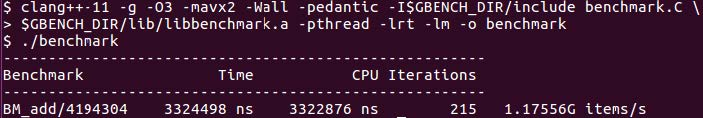
\includegraphics[width=0.9\textwidth]{content/1/chapter3/images/2.jpg}\\
Figure 3.2
\end{center}

So far, we cannot conclude much from this experiment, other than the modern CPUs are fast: they can add two numbers in less than a nanosecond. If you're curious, you can explore other operations at this point: subtraction and multiplication take exactly as much time as addition, while integer division is rather expensive (three to four times slower).

In order to analyze the performance of our code, we have to look at it the way the processor sees it, and there is a lot more going on here than the simple addition. The two input arrays are stored in memory, but the addition or multiplication operations are executed between values stored in registers (or, possibly, between a register and a memory location, for some operations). This is how the processor sees one iteration of our loop, step by step. At the start of the iteration, the index variable i is in one of the CPU registers, and the two corresponding array elements, v1[i] and v2[i], are in memory:

\hspace*{\fill} \\ %插入空行
\begin{center}
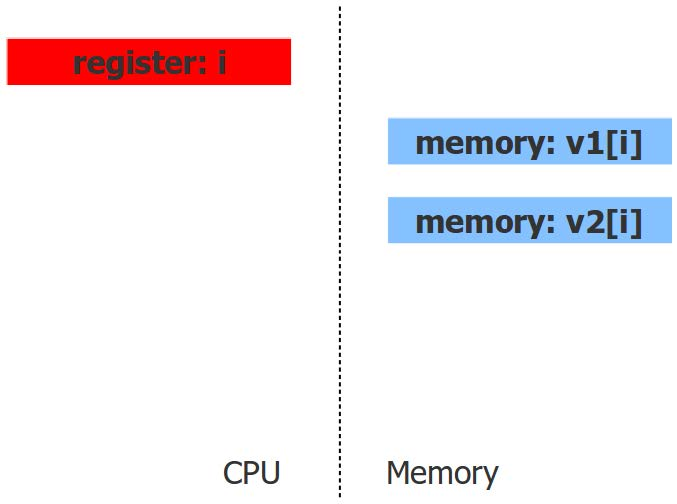
\includegraphics[width=0.9\textwidth]{content/1/chapter3/images/3.jpg}\\
Figure 3.3
\end{center}

Before we can do anything, we have to move the input values into the registers. A register has to be allocated for each input, plus one register for the result. In a given loop iteration, the first instruction will load one of the inputs into the register:

\hspace*{\fill} \\ %插入空行
\begin{center}
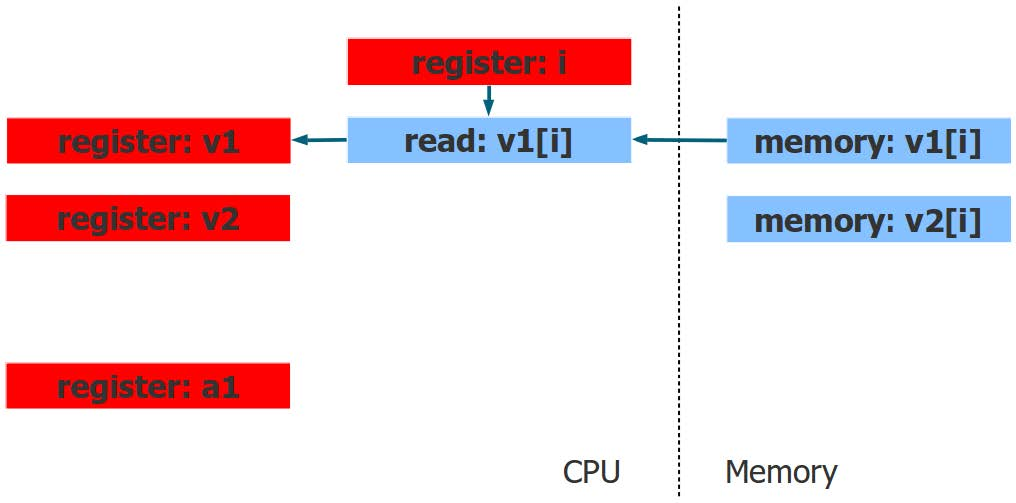
\includegraphics[width=0.9\textwidth]{content/1/chapter3/images/4.jpg}\\
Figure 3.4 – Processor state after the first instruction of the i-th iteration
\end{center}

The read (or load) instruction uses the register containing the index i and the location of the array v1 in memory to access the value v1[i] and copy it into the register. The next instruction similarly loads the second input:

\hspace*{\fill} \\ %插入空行
\begin{center}
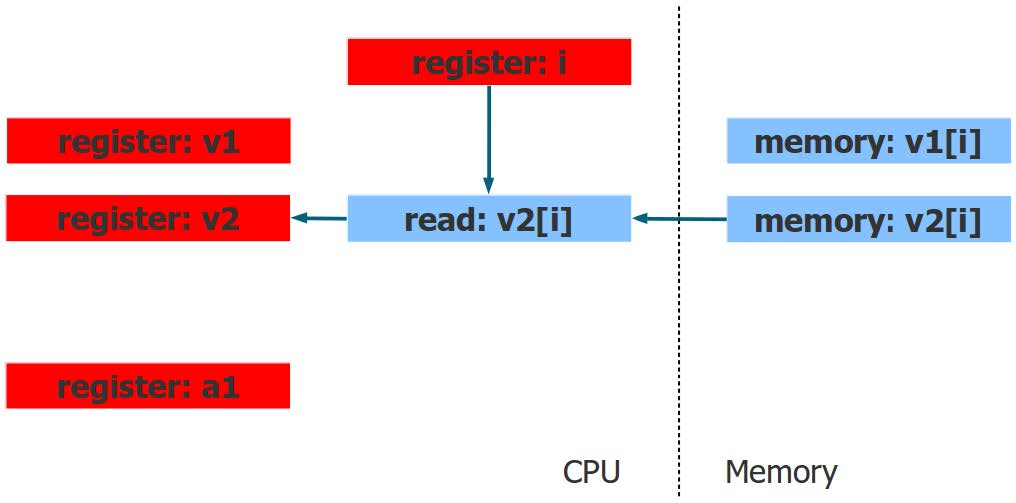
\includegraphics[width=0.9\textwidth]{content/1/chapter3/images/5.jpg}\\
Figure 3.5 – Processor state after the second instruction of the i-th iteration
\end{center}

Now we are finally ready to do the operation such as addition or multiplication:

\hspace*{\fill} \\ %插入空行
\begin{center}
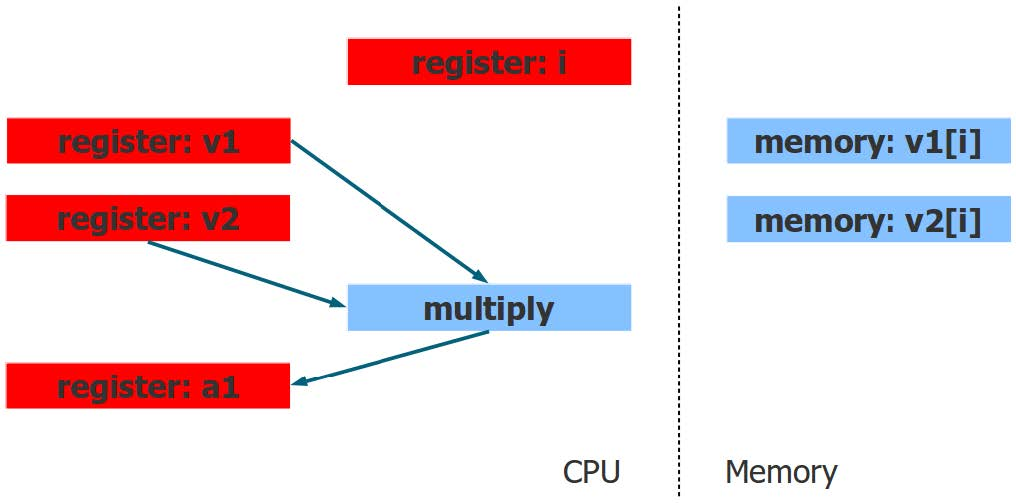
\includegraphics[width=0.9\textwidth]{content/1/chapter3/images/6.jpg}\\
Figure 3.6 – Processor state at the end of the i-th loop iteration
\end{center}

This simple line of code produces all these steps after it is converted into hardware instructions (plus the operations necessary to advance to the next iteration of the loop):

\begin{lstlisting}[style=styleCXX]
a1 += p1[i] + p2[i];
\end{lstlisting}

From the efficiency point of view, we want to focus on that last step: our CPU can add or multiply two numbers in under a nanosecond, not bad, but can it do more? A lot of transistors are dedicated to processing and executing instructions, so they have to be good for something more. Let us try to do two operations on the same values instead of just one:

\begin{lstlisting}[style=styleCXX]
\\ 01_superscalar.C
void BM_add_multiply(benchmark::State& state) {
	… prepare data …
	for (auto _ : state) {
		unsigned long a1 = 0, a2 = 0;
		for (size_t i = 0; i < N; ++i) {
			a1 += p1[i] + p2[i];
			a2 += p1[i] * p2[i];
		}
		benchmark::DoNotOptimize(a1);
		benchmark::DoNotOptimize(a2);
		benchmark::ClobberMemory();
	}
	state.SetItemsProcessed(N*state.iterations());
}
\end{lstlisting}

If an addition takes one nanosecond and a multiplication takes one nanosecond, how long would both take? The benchmark gives us the answer:

\hspace*{\fill} \\ %插入空行
\begin{center}
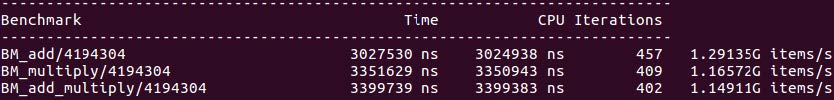
\includegraphics[width=0.9\textwidth]{content/1/chapter3/images/7.jpg}\\
Figure 3.7 – Benchmarks for a single instruction and two instructions
\end{center}

Surprisingly, one plus one equals one here. We can add even more instructions to one iteration:

\begin{lstlisting}[style=styleCXX]
for (size_t i = 0; i < N; ++i) {
	a1 += p1[i] + p2[i];
	a2 += p1[i] * p2[i];
	a3 += p1[i] << 2;
	a4 += p2[i] – p1[i];
}
\end{lstlisting}

The time per iteration is still the same (slight differences are within the accuracy of the benchmark measurement):

\hspace*{\fill} \\ %插入空行
\begin{center}
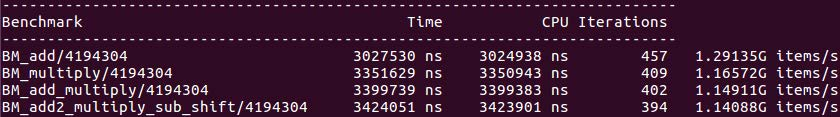
\includegraphics[width=0.9\textwidth]{content/1/chapter3/images/8.jpg}\\
Figure 3.8 – Benchmarks for loops with up to four instructions per iteration
\end{center}

It appears that our view of the processor as executing one instruction at a time needs to be revised:

\hspace*{\fill} \\ %插入空行
\begin{center}
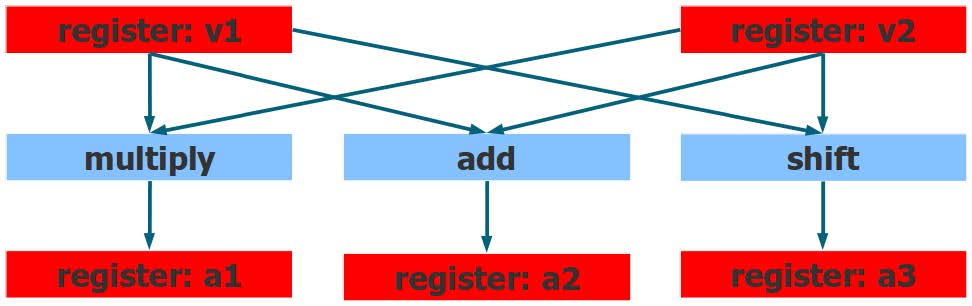
\includegraphics[width=0.9\textwidth]{content/1/chapter3/images/9.jpg}\\
Figure 3.9 – Processor executing multiple operations in a single step
\end{center}

As long as the operands are already in the registers, the processor can execute several operations at once. This is known as Instruction-Level Parallelism (ILP). Of course, there is a limit to how many operations can be executed: the processor has only so many execution units capable of doing integer computations. Still, it is instructive to try to push the CPU to its limits by adding more and more instructions to one iteration:

\begin{lstlisting}[style=styleCXX]
for (size_t i = 0; i < N; ++i) {
	a1 += p1[i] + p2[i];
	a2 += p1[i] * p2[i];
	a3 += p1[i] << 2;
	a4 += p2[i] – p1[i];
	a5 += (p2[i] << 1)*p2[i];
	a6 += (p2[i] - 3)*p1[i];
}
\end{lstlisting}

The exact number of instructions a processor can execute depends on the CPU and the instructions, of course, but the previous loop shows a noticeable slowdown compared to the single multiplication, at least on the machine I am using:

\hspace*{\fill} \\ %插入空行
\begin{center}
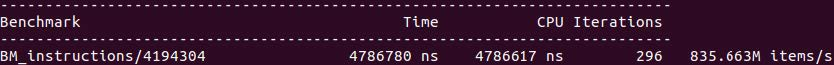
\includegraphics[width=0.9\textwidth]{content/1/chapter3/images/10.jpg}\\
Figure 3.10 – Benchmark of eight instructions per iteration
\end{center}

Now you can appreciate just how inefficient, in terms of the hardware utilization, our original code was: the CPU, apparently, can execute between five and seven different operations per iteration, so our single multiplication wasn't taxing even a quarter of its capabilities. In truth, the modern processors are even more impressively capable: in addition to the integer computation units we have been experimenting with, they have separate floating-point hardware that can execute instructions on double or float values, and the vector processing units that execute MMX, SSE, AVX, and other specialized instructions, all at the same time!

\subsubsubsection{3.3.1\hspace{0.2cm}Visualizing instruction-level parallelism}

So far, our conclusions about the CPU's ability to execute multiple instructions in parallel were based on strong but indirect evidence. It would be good to get a direct confirmation that this is indeed what's going on. We can get such confirmation from the Machine Code Analyzer (MCA), which is a part of the LLVM toolchain. The analyzer takes assembly code as the input and reports a lot of information on how the instructions are executed, what the delays and the bottlenecks are, and so on. We are not going to learn all the capabilities of this advanced tool here (refer to the project home page, \url{https://llvm.org/docs/CommandGuide/llvm-mca.html}, for details). However, we can use it now to see how the CPU executes our operations.

The first step is to annotate the code with the analyzer markup to select which part of the code to analyze:

\begin{lstlisting}[style=styleCXX]
#define MCA_START __asm volatile("# LLVM-MCA-BEGIN");
#define MCA_END __asm volatile("# LLVM-MCA-END");
…
for (size_t i = 0; i < N; ++i) {
MCA_START
	a1 += p1[i] + p2[i];
MCA_END
}
\end{lstlisting}

You don't have to use \#define for the analyzer markup, but I find it easier to remember these commands than the exact assembly syntax (you can save the \#define lines in a header file and include it as needed). Why did we mark for analysis just the body of the loop and not the whole loop? The analyzer actually assumes that the selected code fragment runs in a loop and repeats it for some number of iterations (ten by default). You can try to mark the entire loop for analysis, but, depending on the compiler optimizations, this may confuse the analyzer (it's a powerful tool, but not easy to use or, at the time of writing this, particularly robust).

We can run the analyzer now:

\hspace*{\fill} \\ %插入空行
\begin{center}
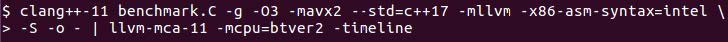
\includegraphics[width=0.9\textwidth]{content/1/chapter3/images/11.jpg}\\
Figure 3.11
\end{center}

Note that we do not compile the code into an executable but rather generate assembly output (-S) in Intel syntax. The output is piped into the analyzer; of the many ways the analyzer can report the results, we selected the timeline output. The timeline view shows each instruction as it moves through the execution process. Let us analyze two code fragments, one with a single operation (addition or multiplication) and the other one with both operations. Here is the timeline for the iteration with just one multiplication (we have removed all the lines in the middle of the timeline):

\hspace*{\fill} \\ %插入空行
\begin{center}
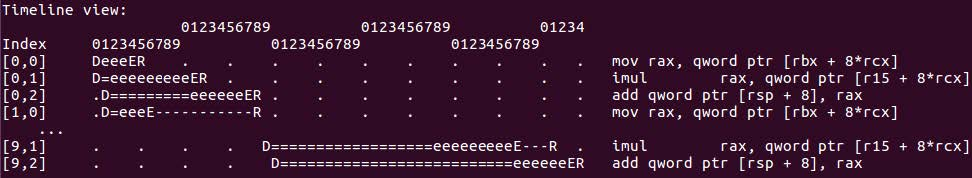
\includegraphics[width=0.9\textwidth]{content/1/chapter3/images/12.jpg}\\
Figure 3.12
\end{center}

The horizontal axis is the time in cycles. The analyzer simulated running the selected code fragment for ten iterations; each instruction is identified by its sequential number in the code and the iteration index, so the first instruction of the first iteration has the index [0,0], and the last instruction has the index [9,2]. This last instruction is also the third instruction of the tenth iteration (there are only three instructions per iteration). The entire sequence took 55 cycles, according to the timeline.

Now let us add another operation that uses the same values p1[i] and p2[i] that we already read from memory:

\begin{lstlisting}[style=styleCXX]
#define MCA_START __asm volatile("# LLVM-MCA-BEGIN");
#define MCA_END __asm volatile("# LLVM-MCA-END");
…
for (size_t i = 0; i < N; ++i) {
MCA_START
	a1 += p1[i] + p2[i];
	a2 += p1[i] * p2[i];
MCA_END
}
\end{lstlisting}

Let us look at the timeline for the code with two operations per iteration, one addition and one multiplication:

\hspace*{\fill} \\ %插入空行
\begin{center}
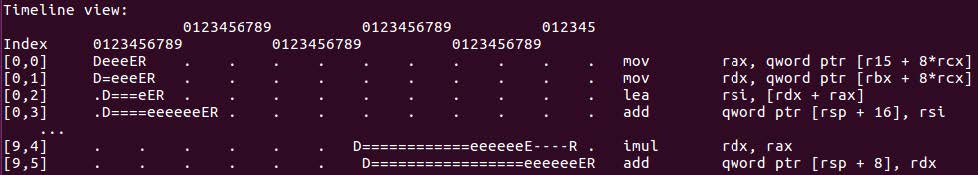
\includegraphics[width=0.9\textwidth]{content/1/chapter3/images/13.jpg}\\
Figure 3.13
\end{center}

There are a lot more instructions executed now, six instructions per iteration (the last instruction has the index [9,5]). However, the duration of the timeline has increased by just one cycle: In Figure 3.12, the timeline ended on cycle 54, whereas in Figure 3.13, it ends on cycle 55. As we have suspected, the processor managed to execute twice as many instructions in the same length of time.

You may have also noticed that for all our benchmarks so far, we have increased the number of operations done on the same input values (add them, subtract them, multiply them, and so on). We have concluded that these extra operations are free as far as the runtime is concerned (up to a point). This is an important general lesson to learn: once you have some values in registers, adding a computation on the same values probably won't cost you any performance unless your program was already extremely efficient and was stressing the hardware to the limit. Unfortunately, the experiment and the conclusions are of limited practical value. How often does it happen that all your computations are done just on a handful of inputs at a time, the next iteration uses its own inputs, and you can find some more useful computations you can do on the same inputs? Not quite never, but rarely. Any attempt to extend our simple demonstration of the CPU's computational power is going to run into one or more complications. The first one is the data dependency: the sequential iterations of the loop are usually not independent; instead, each iteration needs some data from the previous iterations. We will explore this situation in the next section.

















